\documentclass[tikz,border=7pt]{standalone}
\usepackage{amsmath,amssymb}
\usetikzlibrary{arrows.meta,patterns,decorations.markings,calc}
\tikzset{outline/.style={line width=.7pt,line cap=round,line join=round},
 map/.style={outline,-{Stealth[length=2.1mm,width=1.5mm]}},
 point/.style={circle,draw,fill=white,inner sep=1.4pt,line width=.6pt},
 along/.style={postaction={decorate},decoration={markings,mark=at position .52 with {\arrow{Stealth[length=1.8mm,width=1.2mm]}}}}}
\begin{document}
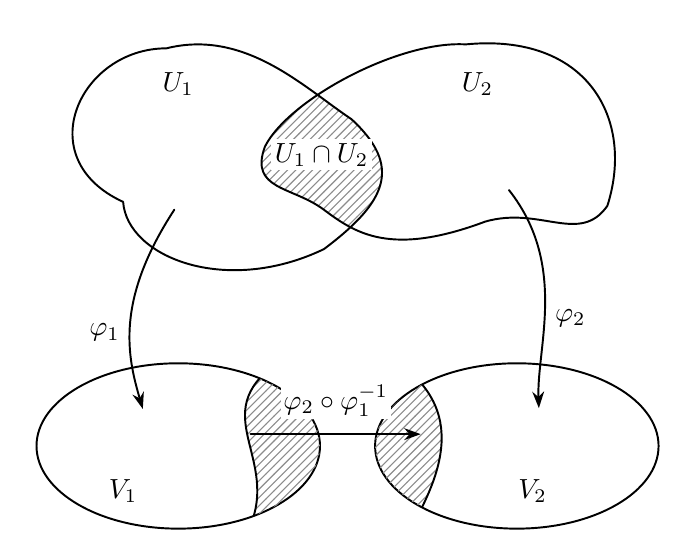
\begin{tikzpicture}[font=\normalsize]

\def\leftregion{(-.15,2.15) .. controls (-1.4,1.55) and (-2.65,2.05) .. (-2.7,2.75) .. controls (-3.9,3.3) and (-3.25,4.7) .. (-2.15,4.7) .. controls (-1.15,4.95) and (-.4,4.2) .. (.2,3.8) .. controls (.85,3.2) and (.65,2.75) .. (-.15,2.15) -- cycle}
\def\rightregion{(-.9,3.45) .. controls (-.6,4.05) and (.8,4.8) .. (1.65,4.75) .. controls (3.2,4.9) and (3.8,3.8) .. (3.45,2.7) .. controls (3.1,2.2) and (2.6,2.7) .. (1.9,2.5) .. controls (.7,2.05) and (.25,2.35) .. (-.15,2.65) .. controls (-.55,2.95) and (-1.1,2.9) .. (-.9,3.45) -- cycle}
\begin{scope}\clip \leftregion;\fill[pattern=north east lines,pattern color=black!45] \rightregion;\end{scope}
\draw[outline] \leftregion;\draw[outline] \rightregion;
\node at (-2,4.25) {$U_1$};\node at (1.8,4.25) {$U_2$};
\node[fill=white,inner sep=1.5pt] at (-.18,3.35) {$U_1\cap U_2$};
\draw[outline] (-2,-.35) ellipse (1.8 and 1.05);
\draw[outline] (2.3,-.35) ellipse (1.8 and 1.05);
\begin{scope}\clip (-2,-.35) ellipse (1.8 and 1.05);
\fill[pattern=north east lines,pattern color=black!45] (-.75,.7) .. controls (-1.65,.05) and (-.7,-.5) .. (-1.1,-1.4) -- (.1,-1.4) -- (.1,.8) -- cycle;
\draw[outline] (-.75,.7) .. controls (-1.65,.05) and (-.7,-.5) .. (-1.1,-1.4);\end{scope}
\begin{scope}\clip (2.3,-.35) ellipse (1.8 and 1.05);
\fill[pattern=north east lines,pattern color=black!45] (.8,.7) .. controls (1.65,.1) and (1.35,-.7) .. (.95,-1.4) -- (.1,-1.4) -- (.1,.8) -- cycle;
\draw[outline] (.8,.7) .. controls (1.65,.1) and (1.35,-.7) .. (.95,-1.4);\end{scope}
\node at (-2.7,-.92) {$V_1$};\node at (2.5,-.92) {$V_2$};
\draw[map] (-2.05,2.65) .. controls (-2.8,1.5) and (-2.65,.8) .. (-2.45,.12) node[pos=.55,left] {$\varphi_1$};
\draw[map] (2.2,2.9) .. controls (2.95,1.95) and (2.55,.9) .. (2.58,.13) node[pos=.56,right] {$\varphi_2$};
\draw[map] (-1.08,-.2) -- (1.08,-.2) node[midway,above=5pt,fill=white,inner sep=1pt] {$\varphi_2\circ\varphi_1^{-1}$};

\end{tikzpicture}
\end{document}
